\chapter{Complex Networks}
\label{chap:complexnetworks}

%Often, the term ``network'' is associated only with computer

%Often, when people hear the term ``network'', they think only of technological examples, such as computer networks.
%Such networks are only a subset of a much larger field of study: that of complex networks.
%The study of complex networks dates back decades, including analysis of biological or social networks \cite{wang2003complex} \cite{newmannetworks}.
%Technological networks, and VANETs by extension, are only a subset of that much larger field of study.
%
%Trust issues and their solutions are an important aspect of the study of complex networks, and of social or technological networks in particular.
%Each different type of network requires a specific approach to trust, according to the features that distinguish it from others.
%It is interesting to review the solutions proposed for social networks and technological networks in general, and then narrow down on how dynamic networks, and VANETs in particular, are handled.
%Despite the differences, there are some concepts that overlap across most types of networks.


Complex networks can describe many systems which are observed in nature and society through a collection of \textit{vertices} (or \textit{nodes}) and \textit{edges} \cite{newmannetworks}.
They can be comprised of palpable components (such as computers and cables), somewhat abstract entities (such as the World Wide Web's collection of webpages and URLs), or both (like the people and relationships that form a social network).
The study of networks is tied to graph theory, since graphs are a useful way to generate models of networks, and therefore many concepts of the two fields overlap.
Mathematical, computational and statistical concepts developed for graphs can be translated to be useful for a variety of different types of networks, like, for example, finding articulation vertices in a graph to locate bandwidth bottlenecks in a computer network.

Complex networks are generally divided into four categories \cite{newmannetworks}:

\begin{enumerate}
	\item \textbf{Technological Networks} are grids purposefully engineered to provide services to consumers and/or citizens.
	 	The primary examples of these networks are the Internet, the telephone network, power grids, transportation and delivery networks.
	 	A commonly studied type of technological network are Mobile Ad-hoc Networks (MANETs).
		Although not of widespread use, MANETs can provide a way to create a network without pre-existing infrastructure, as long as each device is equipped with the proper hardware and software.
		Trust issues in technological networks and MANETs are detailed in \autoref{section:trusttechnological}.
		VANETs, which are special types of MANETs, are introduced in \autoref{chap:vanets}, along with several details regarding trust in those types of networks.
	\item \textbf{Social Networks} are formed of relationships between people, or groups of people.
		These relationships can be familiar, friendships, acquaintance, etc.
		For the purposes of this work, the most relevant type of relationship is that of trust.
		The details surrounding trust relationships in social networks are shown in \autoref{section:trustsocial}.
	\item \textbf{Information Networks} are the ones in which nodes are pieces of data or information and the edges are the connections between those pieces.
		Often, information networks are directly associated with technological or social networks.
		For instance, while the World Wide Web is an information network (in which the nodes are webpages and the edges are the links that users click on to navigate), it relies on the Internet, as it contains the physical infrastructure that makes the web possible.
		Online social networks can also be classified as information networks, since their nodes are actually information about people rather than the people themselves.
		Trust in information networks can be observed in some instances, like peer-to-peer networks [cite], although its usages are not relevant for this work.
	\item \textbf{Biological Networks} are the networks found in nature.
		Their nodes can be chemicals, cells, animals, groups of lifeforms, and more.
		An example is the brain, which contains a neural network formed by neurons, cells which enable information processing; connections in the network represent signals that are sent from one neuron to another.
		Another instance of biological networks are food chains, categorized as ecological webs.
		Species of animals are the nodes, while the predation of other species form the edges.
		In biological networks, it is difficult to clearly define trust, since nodes may not have any sort of awareness or intelligence (such as cells or proteins).
		Regardless, the study of trust in biological networks is not relevant for this proposal.
		
\end{enumerate}

%While issues of trust have been studied on most types of networks, this work will emphasize on social and technological networks, because previous study on both can provide useful insights towards trust in vehicular networks.
%It is clear that VANETs are part of technological networks; in this work, however, it is also argued that vehicular networks present features usually attributed to social networks.
%Therefore, further details, as well as trust issues and proposed solutions, for both social and technological networks are presented in this chapter.

In most networks, trust can be a useful tool to aid the security and safety of its members.
Therefore, the study of the concept and applications of trust is an important part of the study of networks. 

Trust is a concept studied in fields such as psychology and economics, with specific definitions.
In complex networks, under the perspective of computer science, it is a measure of one entity's confidence that another will behave properly and provide valid and/or meaningful data \cite{sherchan2013survey}.
What follows is the basis of how a network can be modelled using a graph and how a trust model can be applied to it.

Consider an undirected graph $G = (V,E)$, which models one complex network of any kind.
The vertices are the members of the network (computers, humans, etc.) and each edge represents a pair of vertices' ability to exchange data freely.
This graph represents the network's \textit{topology}, that is, the basic structure of the network.
Then, there is also a directed graph $T = (V, O)$, called a \textit{trust graph}.
$T$ contains the same nodes as $G$, although its edges represent the degree of trust (or opinion) each node has towards another.

There are two main ways to describe the edges in $O$: they can be binary, either existing when there is trust or not otherwise, or they can hold a specific trust value within a certain range.
This means the shape of $T$ is not necessarily similar to that of $G$.
For instance, two people can have contact with each other but not maintain a trust relationship, thus altering the layout of the trust graph compared to the network topology.

In the following two sections of this chapter, trust in the contexts of social and technological networks is further explained.
Both types of network can be fitted into the model above, but contain distinct features that demand closer examination.
Furthermore, features of both are relevant when analyzing network structure and trust graphs for vehicular networks, which is expanded upon in \autoref{chap:vanets}.

%As this work relates to trust issues in complex networks, it is interesting to further examine social networks and the importance of trust within them.
%While the end result of the study will be applied to technological networks, certain aspects of social networks provide useful analogies to trust management in other kinds of networks.

\section{Trust in Social Networks}
\label{section:trustsocial}
There are two types of social networks: real-world ones formed by relationships between people, and online ones that attempt to abstract the former into a digital environment.
Examples of the first one are all around, present in any family, workplace, school or group of friends \cite{newmannetworks}.
Online social networks started by connecting people who already knew each other and giving them an additional form of interaction (analogous to what telephones and email did before), but, today, it is not unusual for people to form relationships with others whom they have only met online. 

In a traditional social network, it is simple to perceive how trust is relevant and how it works, since trust relationships between people are used on a daily basis to make decisions.
When adapted to a digital environment, these social relationships can be used to automatically increase the relevance of certain information.
For instance, upon reading an online review for a certain product, a user will be more likely to accept the review's conclusion if it was written by a close friend than if it were written by a stranger.
Social trust is a way of estimating how much a certain recommendation will lead to a positive outcome \cite{golbeck2006inferring}. 

The absence of trust or the presence of distrust have consequences as well.
Both in the real world and online, information which comes from a stranger is received with uncertainty; there is no reason to trust the sender, so the data itself must be analyzed and compared to other sources in order to judge whether or not it may be trusted.
When one person actively distrusts another (that is, the person believes the other is malicious or uninformed), receiving data from the untrustworthy source will be actively avoided.
In online social networks, for example, one user can ``block'' another in order to avoid seeing anything from the other.

%Furthermore, if the review was written by a person who the user knows to be malicious or uninformed, its contents will be even less relevant.

Social networks also have the property of carrying trust from one relationship to another:
information shared by a close friend of a person might be considered almost as trustworthy as some collected by the person him or herself.
Therefore, it is possible to model social trust relationships as a graph, in which nodes represent people and edges represent a certain degree of trust \cite{newmannetworks}.
Expanding on that property, there is the concept friends of friends \cite{boissevain1974friends}.
If, for example, nodes $A$ and $B$ have mutual trust and are considered friends, then it is reasonable to assume that some of $A$'s trust for $B$ carries over to other nodes that enjoy mutual trust with $B$.
In other words, a friend of a friend can be considered more trustworthy than the average stranger.
This property is similar, although not identical, to transitivity, since trust is diminished for each extra step an origin node needs to reach a destination, and there is also the possibility that one node distrusts another even if they share a mutual friend.
Naturally, social trust is not commutative ($A$ trusting $B$ does not imply that $B$ trusts $A$).

In general, social networks' topology and trust graphs are mostly static.
Although friendships are formed and ended frequently (i.e. the topology is dynamic), those connections do not disrupt the general shape of the network, because members of the network will usually have other friends whose relationships remain stable.
Even if a certain person's trust integrity is compromised due to a specific incident, that person's friends are not necessarily deemed untrustworthy, preserving part of the trust graph.
While positive trust is often tied to the social topology, it is not always the case: one example is two work colleagues who may have a professional relationship, but wouldn't trust each other on other matters; another is the trust people place in authority figures without necessarily having met. 
\autoref{fig:social_network} shows an example of a small social network containing a family and an office. 

In \autoref{section:socialvanets}, the argument is made that VANETs can be considered social networks in several occasions and how this can be used to develop trust in vehicular networks. 

%\begin{figure}[h]
%    \centering
%    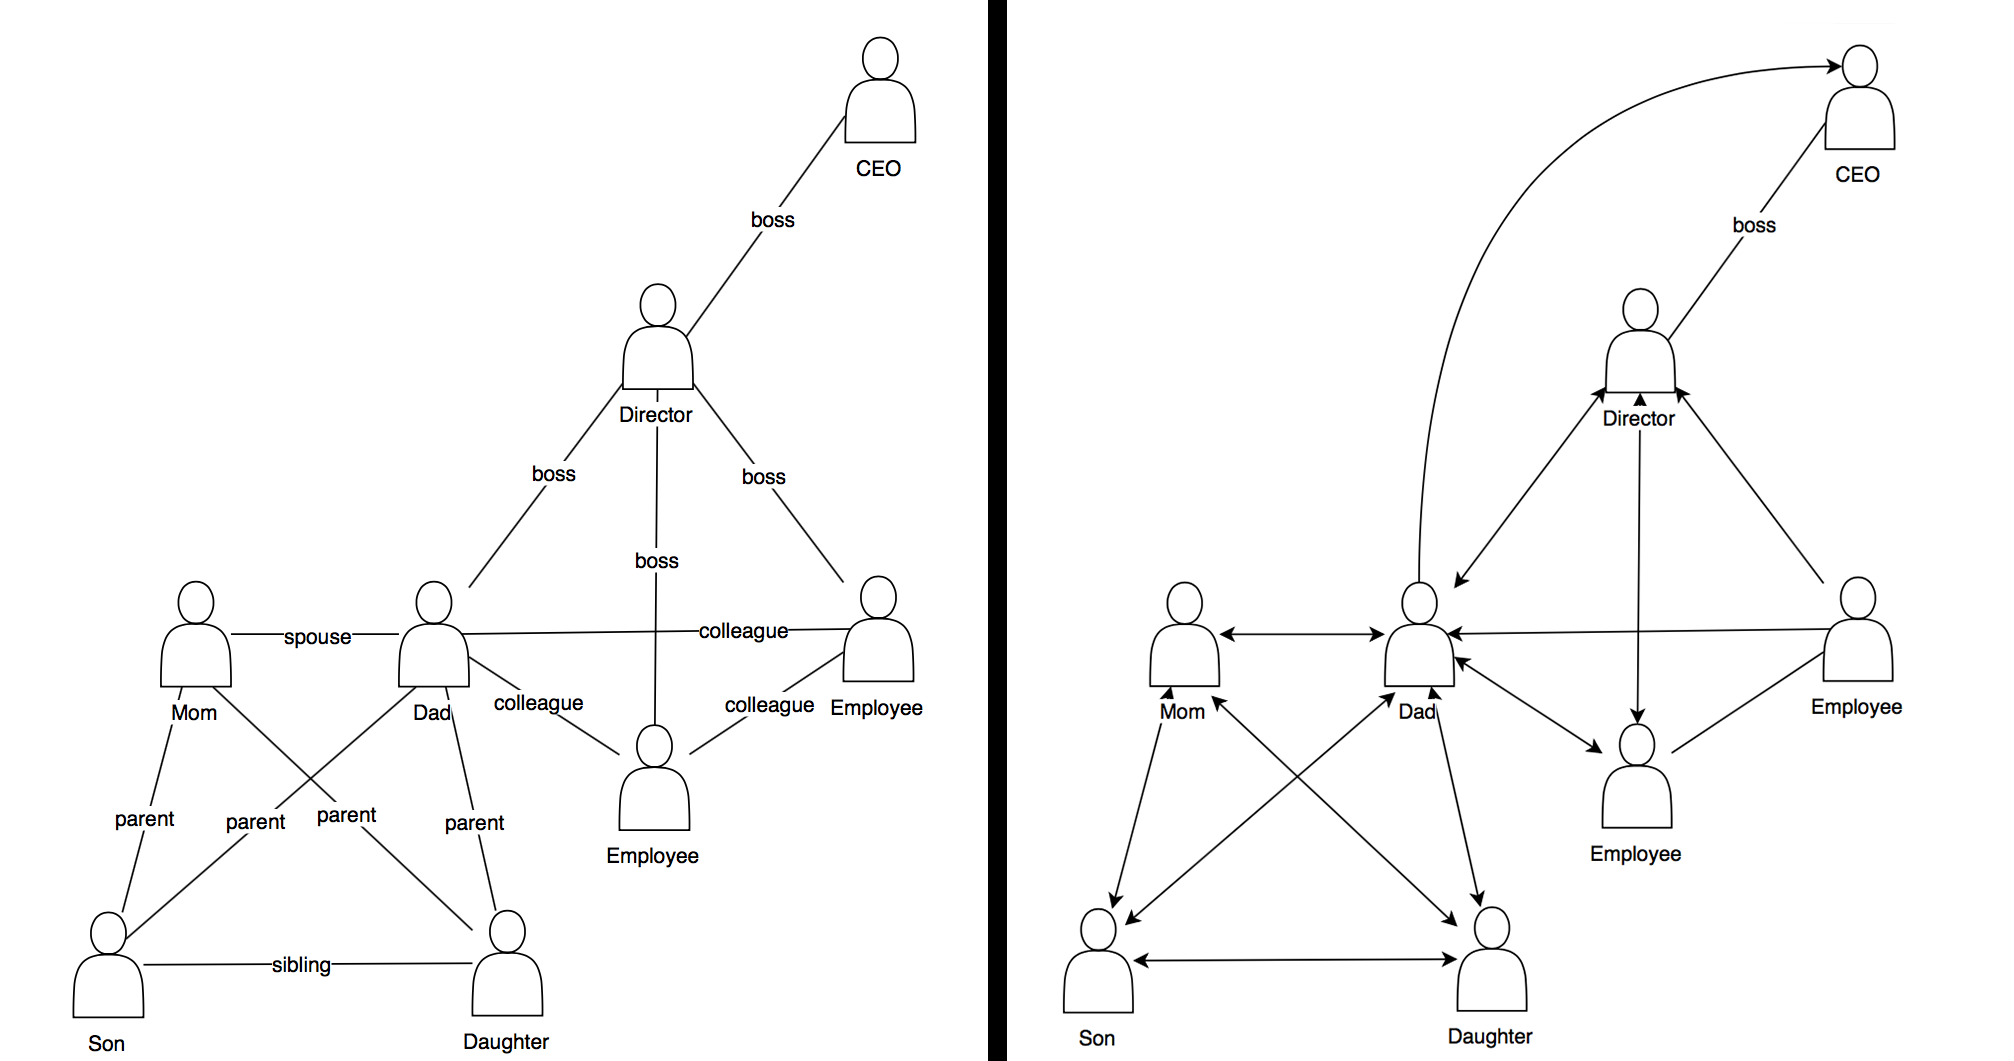
\includegraphics[width=1.0\textwidth]{images/socialnetwork.png}
%    \caption{Example of a topology graph and a trust graph in a social network.}
%    \label{fig:social_network}
%\end{figure}

\begin{figure}
\begin{subfigure}{0.5\textwidth}
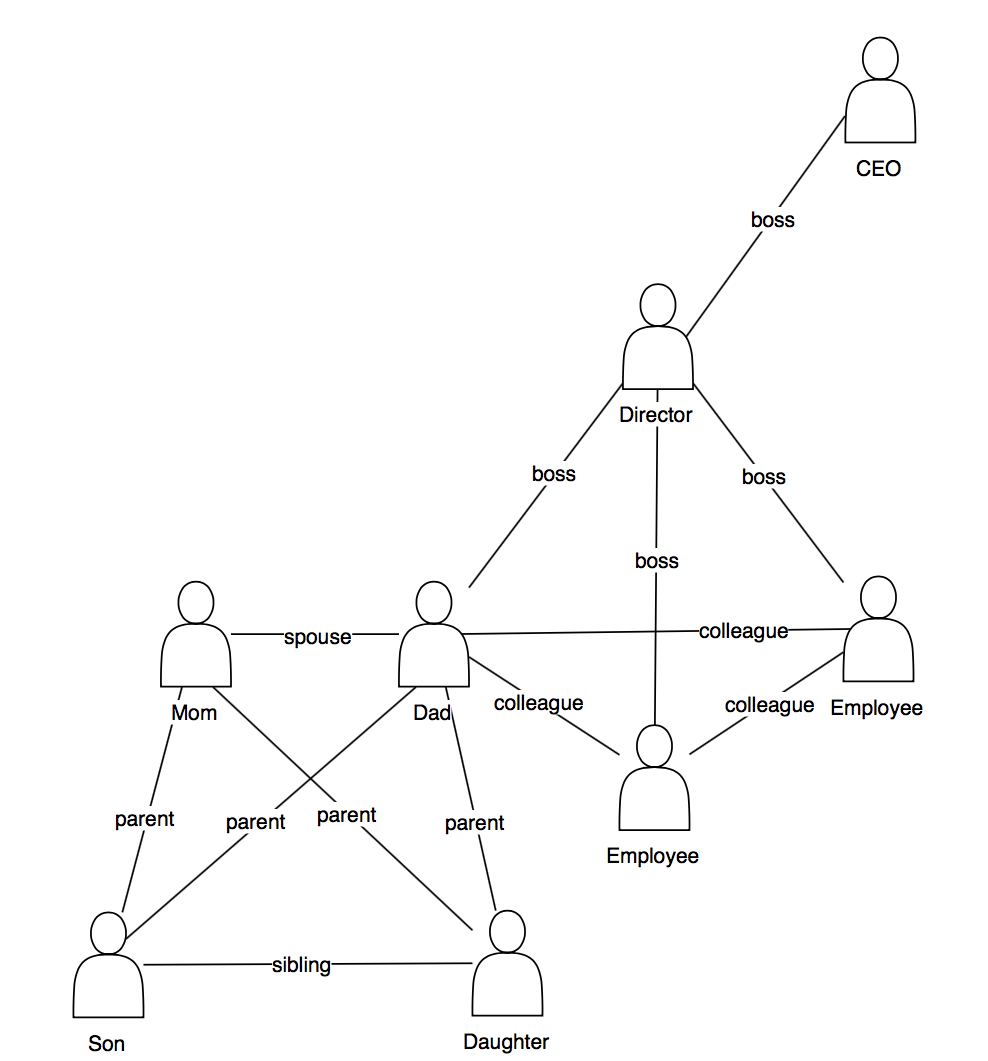
\includegraphics[width=\linewidth]{images/socialnetwork_topology.png}
\caption{Topology graph} \label{fig:2_1a}
\end{subfigure}
\hspace*{\fill} % separation between the subfigures
\begin{subfigure}{0.5\textwidth}
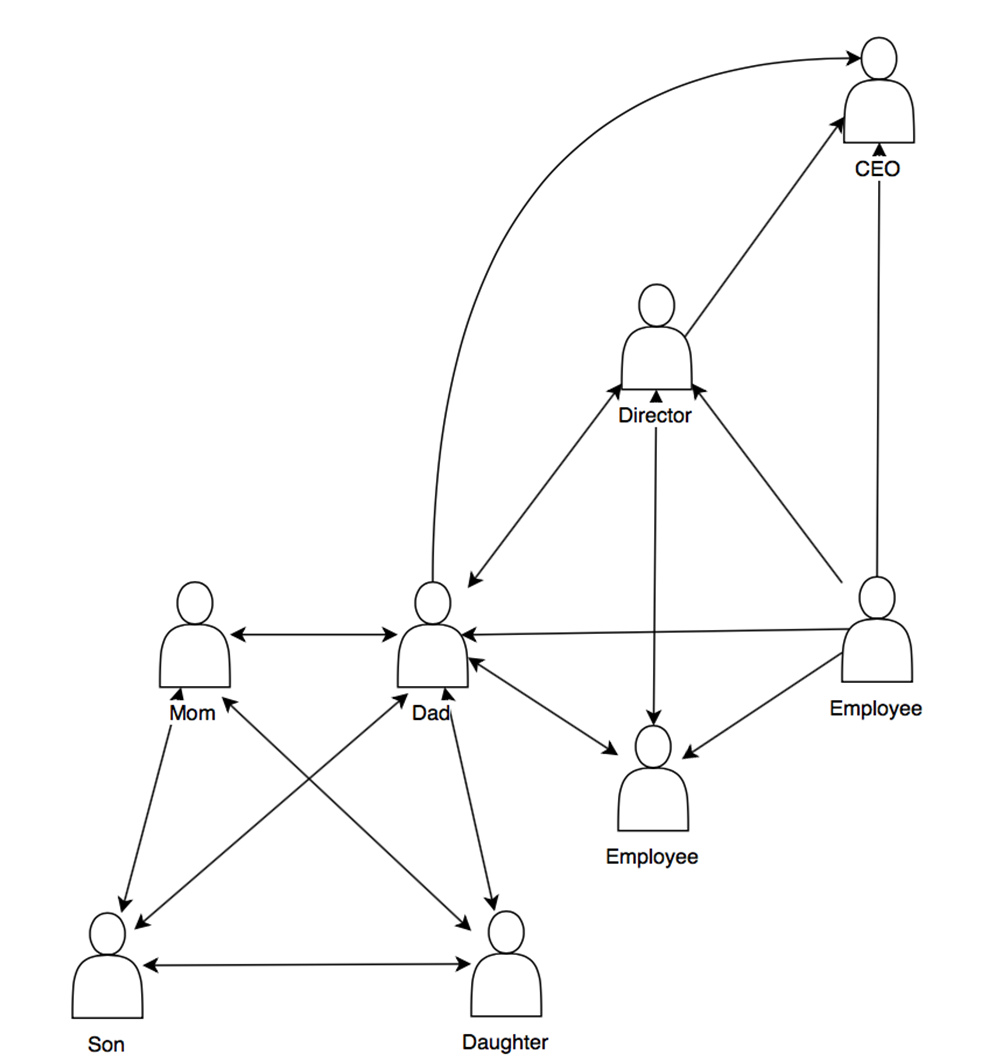
\includegraphics[width=\linewidth]{images/socialnetwork_trust.png}
\caption{Trust graph} \label{fig:2_1b}
\end{subfigure}
\caption{Example of a topology graph and a trust graph in a social network.} \label{fig:social_network}
\end{figure}

%\begin{figure}[htbp]
%\subfloat[Topology graph]{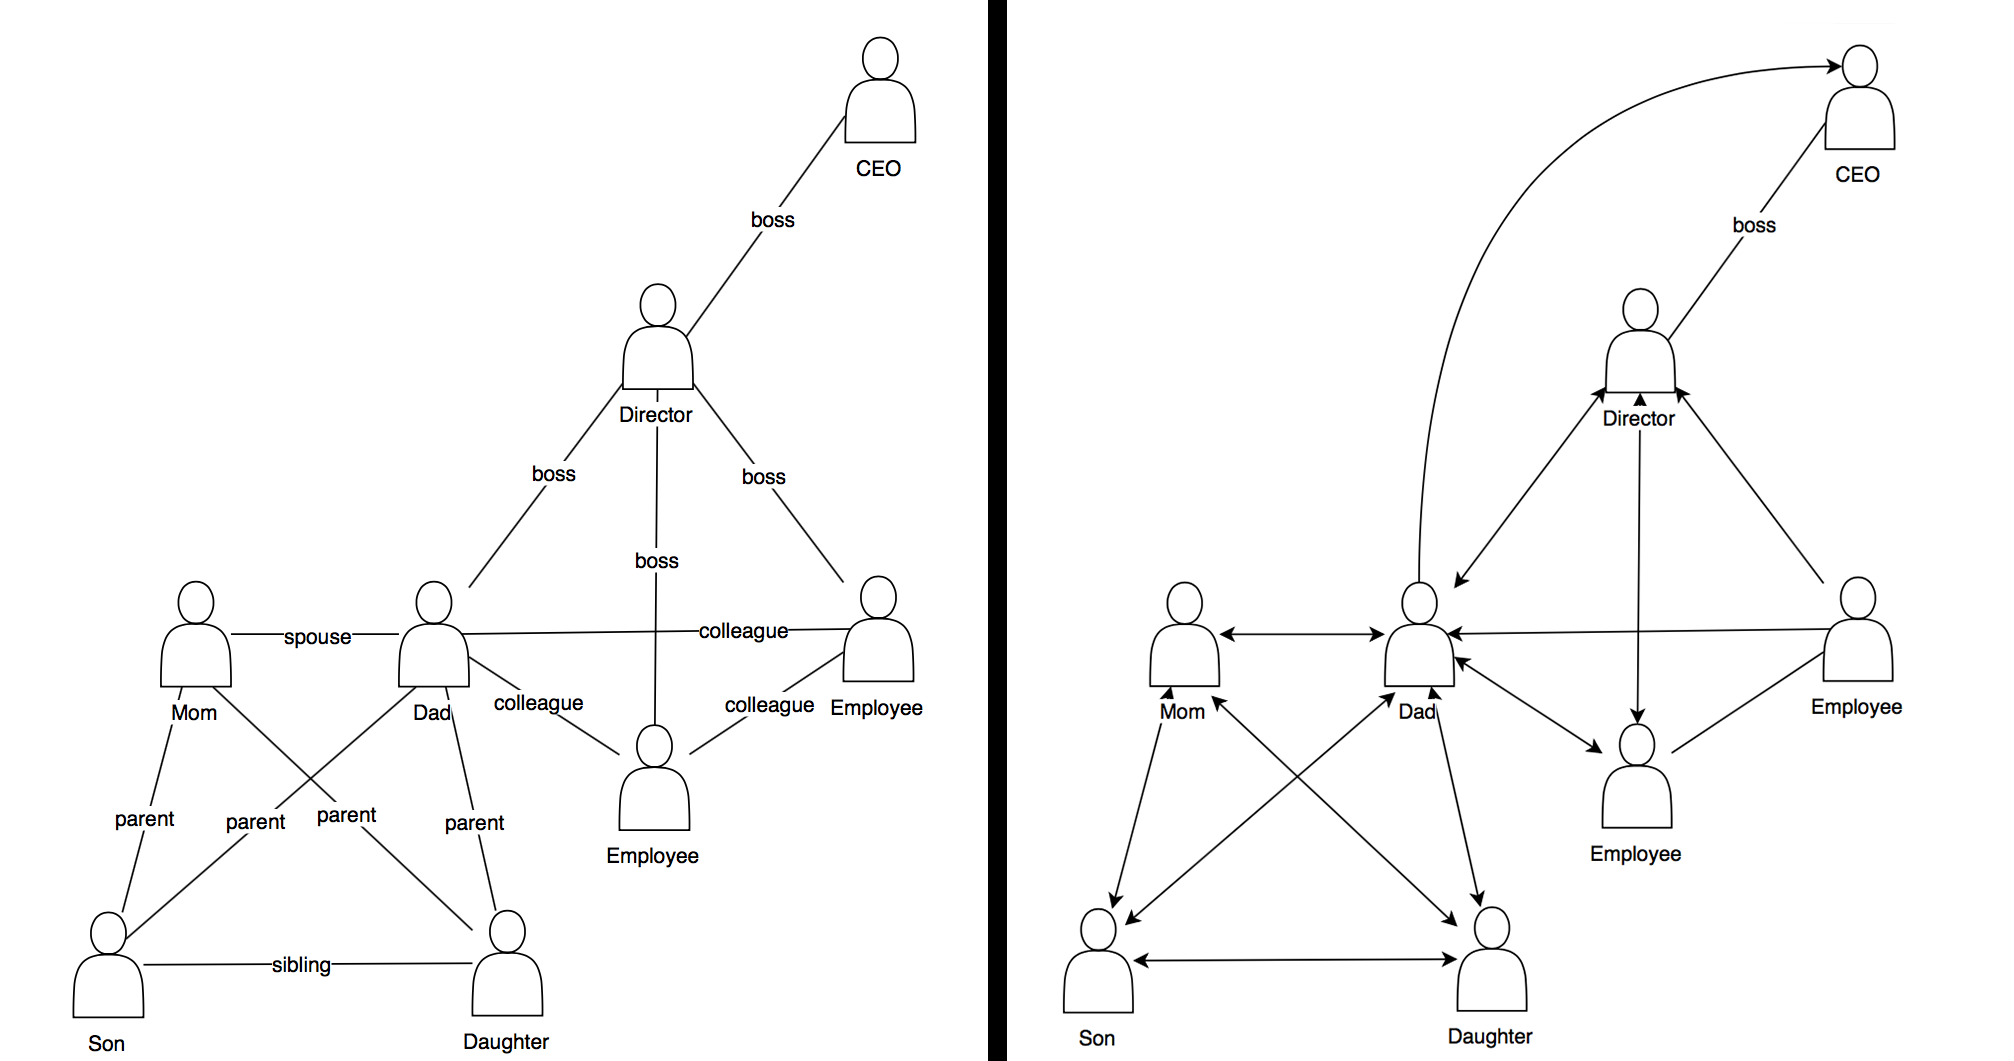
\includegraphics[0.5\textwidth]{images/socialnetwork.png}}
%\subfloat[Trust graph]{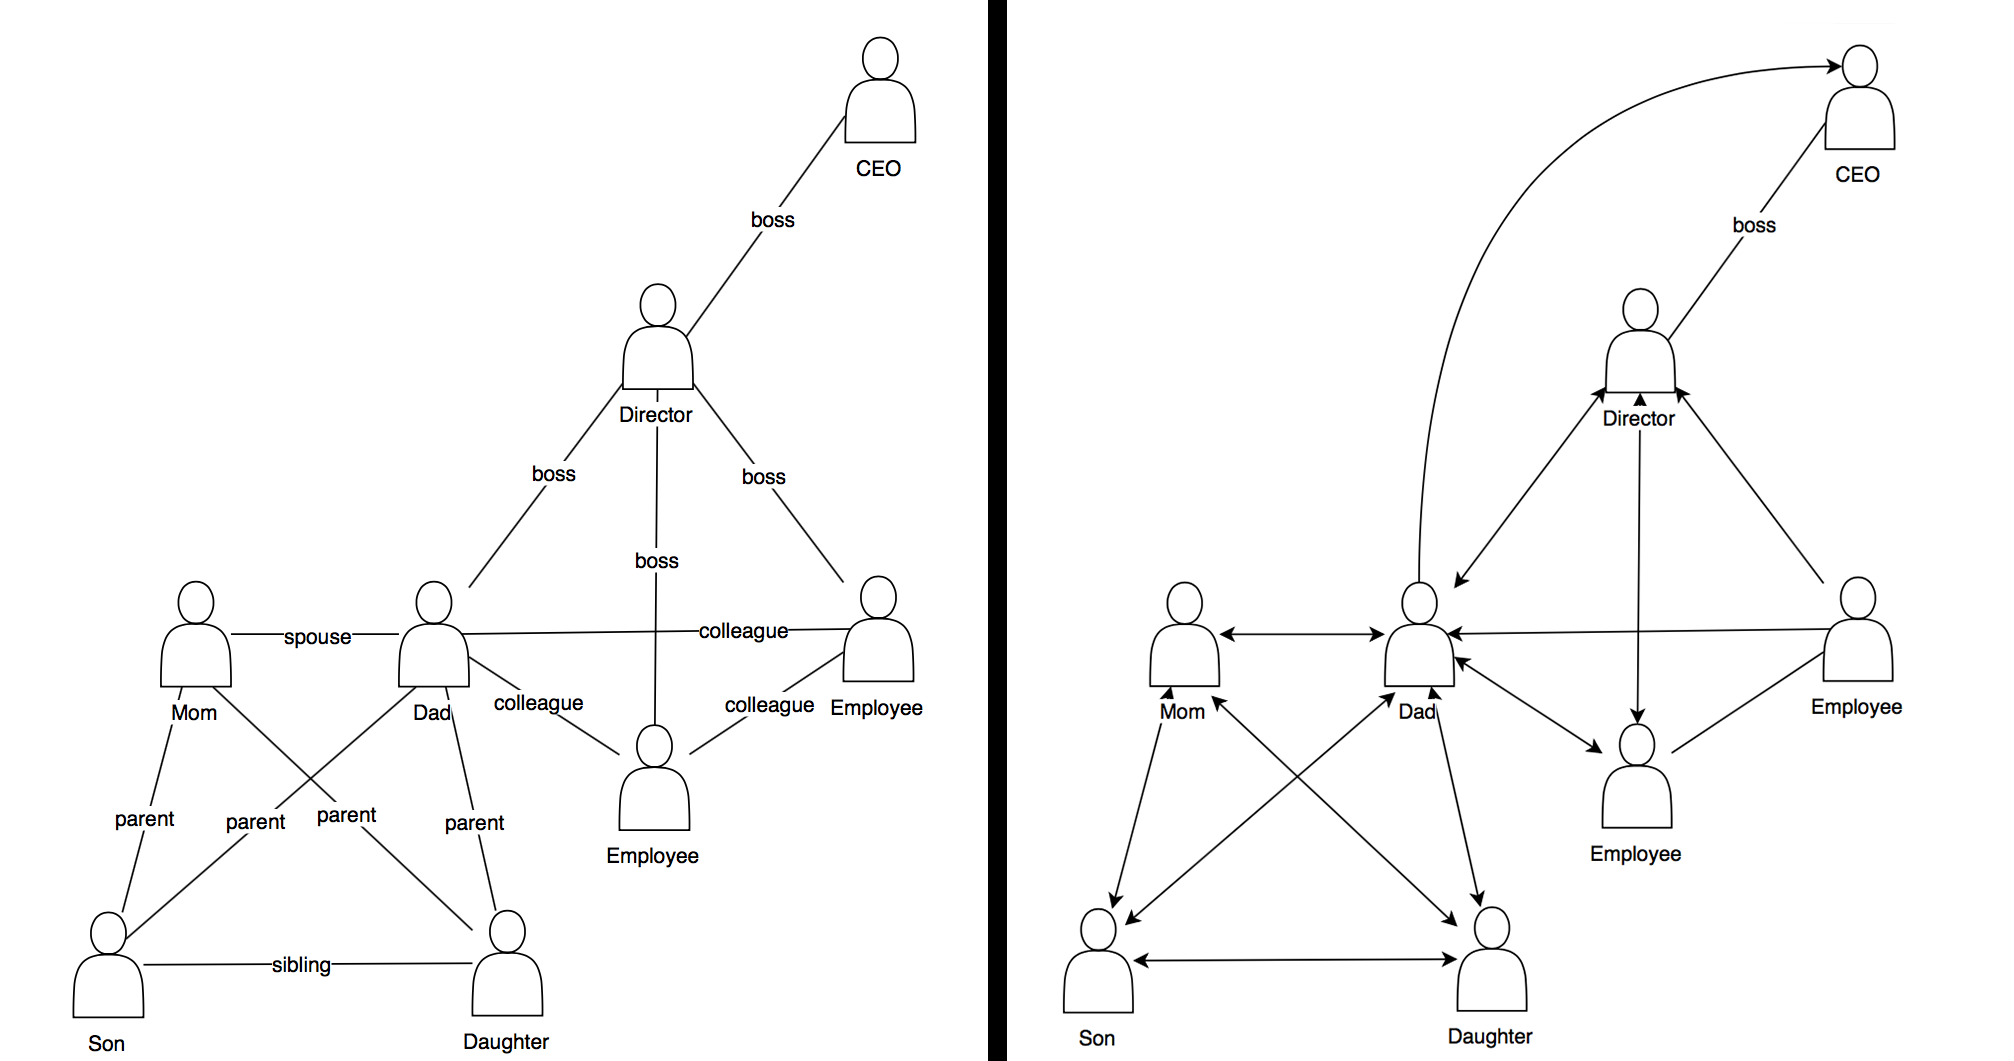
\includegraphics[0.5\textwidth]{images/socialnetwork.png}}
%\caption{Example of a topology graph and a trust graph in a social network.}
%\end{figure}

%Many works exist regarding trust relationships in complex networks, and in social networks in particular.
%Here, only a few examples will be described, in order to show the general idea of trust research for these types of networks.

\section{Trust in Technological Networks}
\label{section:trusttechnological}
In conventional technological networks, such as the Internet, trust is defined and applied quite differently from social networks since, generally, it is very centralized through services that offer security to users.
Examples of this can be an IP filtering scheme to avoid distributed denial of service (DDoS) attacks or web browser extensions that block requests to domains in a blacklist; a central agent, be it a hosting provider or the extension's publisher, must maintain and update a list of untrustworthy IP addresses or domains.
This means that, in the context of the Internet, trust is often derived from a secondary source: end users and their computers can't be expected to maintain their own blacklists, so they rely on external parties which may provide these lists along with other security services.
Similarly, when a user visits an e-commerce website, they must have some degree of trust on the website or the vendor; in this case as well, third-party services are used to certify the legitimacy of the transaction, based on feedback from other customers.

% In ad-hoc networks, such as vehicular networks, which are detailed in \autoref{chap:vanets}, trust can be handled in very different ways.
While the centralized trust solutions above serve their purpose on the security and privacy of Internet users, they would be too slow to be viable in a dynamic ad-hoc network, which cannot rely on a back-end infrastructure to distribute those lists.
The most common instance of mobile ad-hoc networks, or MANETs, is using mobile devices, such as smartphones, being carried by humans.
Although these networks are dynamic, their mobility is relatively low in relation to the wireless range of the devices — if two people are walking in opposite directions, their phones may communicate for several seconds before they leave each other's range.
Trust solutions for MANETs can use this property to their advantage, since it allows one node to test another and check several of the messages sent between them.

% As is the case with social networks, the topology and trust graphs of MANETs are distinct, but 

Ad-hoc networks require a decentralized approach to trust management; each member of a network has its own opinions about other members, and these opinions can change over time.
For these opinions to be generated and updated, two nodes must have had previous contact with each other, or derive trust from a third, intermediary, node.
Hence, there is the correlation between the trust graph and the topology graph of the network.
Since MANETs are dynamic, the graph that represents one network's topology is frequently changing and, with that, the opportunities to create and update trust relationships also changes.
%For two nodes to have a trust relationship at all, the topology must changed in a way so that they are neighbors to each other, or close enough that asking for a third node's
In networks in which nodes can meet more than once, it might be valuable to store information from previous encounters to use in the future, although this process can be too slow or resource-consuming to be viable in certain devices; by doing this, the trust graph maintains edges between nodes that are no longer connected in the topology.

% Ad-hoc networks, such as MANETs and VANETs, are the ob


%For this work, it is necessary to examine closely the case of mobile ad-hoc networks, since it is in that category that VANETs 





%Depending on how the network is structured and its use-cases, it may or not be useful to store these trust values for later use.

%With social networks, the graph that represents relationships 

%With MANETs, however, the graph that represents trust relationships amongst network members is 

%However, while social networks are mostly static, the topology of a MANET changes frequently as nodes move around.
%[Perhaps this is a good place to mention trust vs. trust management]
%Nodes must be able to handle trust with its immediate neighbors for any given moment, so it can properly filter out potentially malicious data.
%In networks in which nodes can meet more than once, it may be valuable to store information from previous encounters to use in the future, although this process can be too slow or resource-consuming to be viable in certain devices.


Another important aspect of trust in ad-hoc networks is that information is, generally, uncertain and incomplete \cite{baras2005cooperation}.
That is, since nodes form their own model and opinions of the surrounding network, it is unlikely that this data will be certain and accurate with reality.
For this reason, it is also possible to use data gathered by neighboring nodes to complement the model.
This data itself is subject to the trust evaluation of the neighbors, but it is crucial to better approximate the trust values of other nodes.
Incompleteness is an inherit trace of MANETs, since it is entirely possible for nodes to be too distant to communicate, and only occasionally come into contact.

Finally, MANETs must consider the processing and battery limitations of the devices that integrate it.
Nodes may disable wireless communications to save power and therefore become uncooperative, or it may be too slow to be a reliable source of information.

There are few examples of MANETs implemented for consumer devices.
Two examples are networks created to quickly share data between devices using Wi-Fi or Bluetooth \cite{krochmal2014discovery}, or ones that allow for multiplayer gaming sessions amongst multiple nearby devices \cite{sasaki2011wireless}.
In both cases, there is no need for a complicated system-level trust model, since those activities involve active participation from the users wielding the device (that is, the user chooses whether or not to communicate with other devices); rather, the trust relationship occurs socially amongst the users themselves.

Naturally, VANETs are an instance of MANETs and therefore share some of the same features.
However, the topology of vehicular networks is very different from standard ad-hoc networks, and possible trust solutions are accordingly also distinct.

\begin{figure}
\centering

\begin{subfigure}{0.5\textwidth}
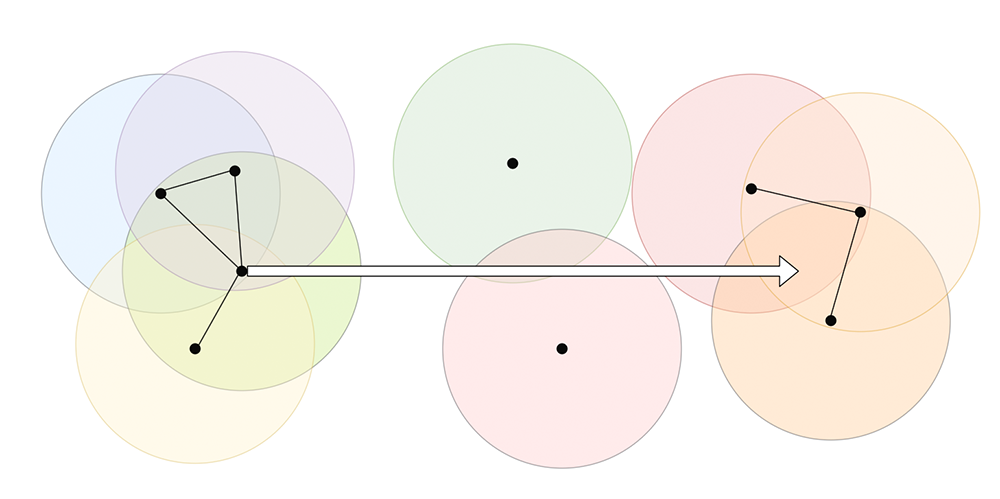
\includegraphics[width=\linewidth]{images/manet_topology_1.png}
\caption{Initial topology and trust graph} \label{fig:2_2a}
\end{subfigure}

\vspace*{\fill} % separation between the subfigures

\begin{subfigure}{0.5\textwidth}
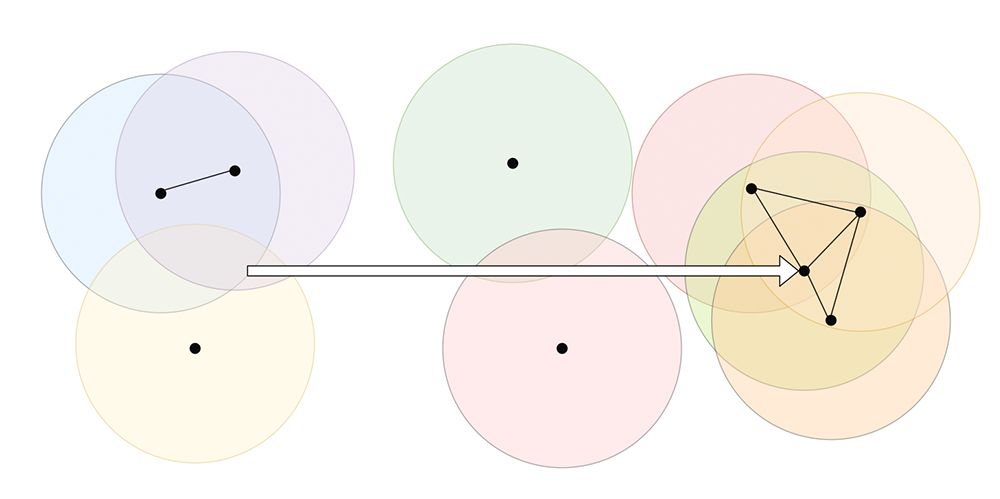
\includegraphics[width=\linewidth]{images/manet_topology_2.png}
\caption{Final topology graph} \label{fig:2_2b}
\end{subfigure}

\vspace*{\fill} % separation between the subfigures

\begin{subfigure}{0.5\textwidth}
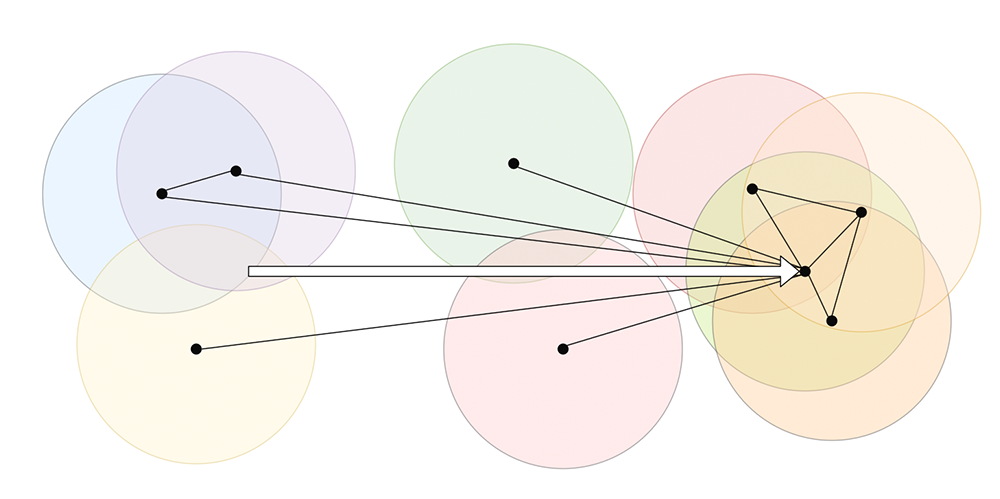
\includegraphics[width=\linewidth]{images/manet_trust.png}
\caption{Final trust graph} \label{fig:2_3b}
\end{subfigure}

\caption{Example of the changes node mobility causes to the topology and trust graphs.} \label{fig:manet}
\end{figure}

%=====================================================